% template cloned from https://gitlab.kit.edu/kit/kastel/sdq/dokumentvorlagen/praesentationen/beamer
% commit: 7960880f39b47ec10eabeed2baf9468fb38312a5 (Mar 4, 2025)

\documentclass[en, navbaroff, handout]{sdqbeamer}
% class options:
% - language: de (default), en
% - navbar can be toggled on (default) / off
% - footer font size: bigfoot (default), smallfoot (KIT layout)
% - font for slide titles: franklin (default) / helvet
% - show lines for alignining content on slides: kitgrid
% - remove animation roll-out: handout (general "beamer" option, not specific for this class)

\grouplogo{} % needs to be empty to be turned off
\groupname{} % empty allows author and title to take more space
%\groupnamewidth{89mm} % default

\title[Subgroup Discovery with Small and Alternative Feature Sets]{Subgroup Discovery with Small and Alternative Feature Sets} % [footer]{title slide}
\subtitle{SIGMOD 2025 | Berlin} 
\author[Jakob Bach]{Jakob Bach} % [footer]{title slide}

\date[2025-06-24]{June 24, 2025} % [footer]{title slide}

%\usepackage{amsmath} % mathematical symbols and equations; apparently pre-loaded
%\usepackage{amssymb} % mathematical symbols; apparently pre-loaded
\usepackage[style=numeric, backend=bibtex]{biblatex}  % original template uses "biber" as backend
\usepackage{booktabs} % nicely formatted tables (with top, mid, and bottom rule)
%\usepackage{graphicx} % plots; apparently pre-loaded
\usepackage{subcaption} % subfigures
\usepackage{tikz} % used for non-float figure positioning
%\usepackage{hyperref} % links and URLs; apparently pre-loaded

\addbibresource{references.bib}

\hypersetup{colorlinks=true, citecolor=kit-blue, urlcolor=kit-blue}
 
\setlength{\leftmargini}{0.6cm} % change default indentation (so first-level items are left-aligned to boxes and slide titles)

\setbeamerfont{itemize/enumerate subbody}{size=\normalsize} % make 2nd-level items' text as large as 1st-level ones (default is \small, as defined in "beamerfontthemedefault.sty")
\setbeamerfont{itemize/enumerate subsubbody}{size=\normalsize} % make 3rd-level items' text as large as 1st-level ones (default is \footnotesize, as defined in "beamerfontthemedefault.sty")

% make bullet points slightly smaller and roughly center them relative to upper-case letters (instead of bottom alignment):
\setbeamertemplate{itemize item}{\raisebox{2.17pt}{\color{kit-green}\footnotesize$\blacksquare$}}
\setbeamertemplate{itemize subitem}{\raisebox{2.17pt}{\color{kit-green}\scriptsize$\blacksquare$}}
\setbeamertemplate{itemize subsubitem}{\raisebox{2.17pt}{\color{kit-green}\scriptsize$\blacksquare$}}

\setbeamercovered{invisible} % can set "transparent" to show later content of animated slide in gray

\begin{document}

\begin{frame}[title white horizontal, kitlogo=rgb]
	% layout options: "white horizontal", "green horizontal", "white vertical", "blue vertical"
	% KIT logo options: rgb, white, black
	\titlepage
\end{frame}

\section{Talk}

\begin{frame}[t]{Subgroup Discovery}
	\begin{itemize}
		\item \textbf{Subgroup discovery:} ``Identifying descriptions of subsets of a dataset that show an interesting behavior''~\cite{atzmueller2015subgroup}
		%JB: unlike typical ML prediction models, need not cover full dataset with one subgroup (there may be multiple ones)
		\begin{itemize}
			\item Language for descriptions typically simple
			%JB: e.g., restrict ranges of numerical features or select particular values of categorical features
			\item `Interesting' according to some objective function
			%JB: notion of subgroup quality
		\end{itemize}
		\pause
		\vspace{\baselineskip}
		\item \textbf{Our scope:} Binary classification with real-valued features
		\begin{itemize}
			\item Tabular dataset $X \in \mathbb{R}^{m \times n}$ (data objects $\times$ features)
			%JB: there also are variants of subgroup discovery that are more like frequent itemset mining, with binary feature values and only value 1 used in subgroup descriptions
			\item Prediction target $y \in \{0, 1\}^m$ (`interesting'/`positive' = 1)
			%JB: in regression, interestingness could refer to low or high values of target
			\pause
			\item Subgroup description: Hyperrectangle
			\item Subgroup quality: Weighted Relative Accuracy
			\begin{itemize}
				\item $\text{WRAcc} = \frac{m_b}{m} \cdot \left( \frac{m_b^+}{m_b} - \frac{m^+}{m} \right)$~\cite{lavravc1999rule}
				%JB: first factor is subgroup size, second is relative accuracy (precision in subgroup vs overall)
				\item \emph{+} $\leftrightarrow$ positive data object, \emph{b} $\leftrightarrow$ in subgroup (box)
			\end{itemize}
		\end{itemize}
		\pause
		\vspace{\baselineskip}
		\item \textbf{Our goal}: Improve interpretability with constraints
		%JB: on selected features
		%JB: despite subgroup descriptions already being simple
		\begin{itemize}
			\item Limit number of features used in subgroup description
			%JB: "small"
			%JB: imagine dataset with 100 dimensions and all are bounded
			%JB: kind of extension to traditional feature selection in ML (one binary decision for each feature; now values play a role)
			\item Find alternative subgroup descriptions
			%JB: "alternative"
			%JB: alternative description for same subgroup, not an alternative subgroup
		\end{itemize}
	\end{itemize}
	\pause[0] % \visible or \onslide did not work, so we reset pause counter to show figure immediately
	\begin{tikzpicture}[remember picture,overlay]
		\node[xshift=-260pt,yshift=-310pt] at (current page.north east) {
			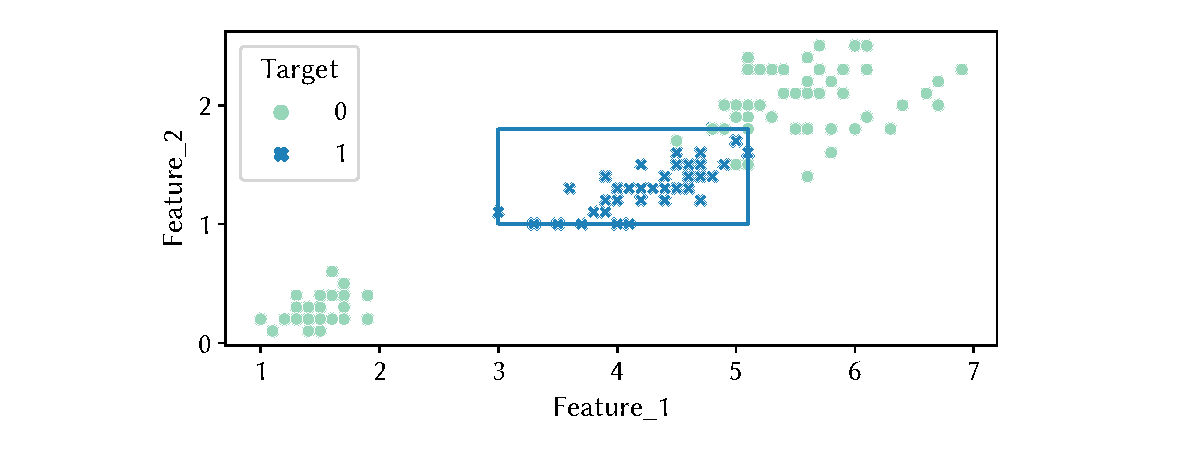
\includegraphics[width=0.45\textwidth, trim=70 15 90 15, clip]{plots/csd-exemplary-subgroup.pdf}
		};
	\end{tikzpicture}
\end{frame}

\begin{frame}[t]{Contributions and Related Work}
	\begin{itemize}
		\item \textbf{Contributions:}
		%JB: formalization, proofs, and experiments
		\begin{itemize}
			\item Formalize subgroup discovery as an SMT (Satisfiability Modulo Theories) optimization problem
			%JB: can be tackled with a solver instead of needing to develop a problem-specific algorithm (which may need further adaptation for particular constraint types)
			\item Formalize two constraint types:
			%JB: the two points mentioned on previous slide
			%JB: all following contributions are for both constraint types each
			\begin{itemize}
				\item Feature-cardinality constraints
				\item Alternative subgroup descriptions
			\end{itemize}
			%JB: besides SMT formalization, also show how to integrate constraints into existing, heuristics subgroup-discovery methods
			\item Analyze computational complexity and show $\mathcal{NP}$-hardness
			%JB: unfortunately, no time for these proofs in this 15-min presentation
			\item Comprehensive experiments
			% will be presented later
		\end{itemize}
		\pause
		\vspace{\baselineskip}
		\item \textbf{Related work:}
		\begin{itemize}
			\item Existing subgroup-discovery methods~\cite{atzmueller2015subgroup, helal2016subgroup, herrera2011overview, ventura2018subgroup} typically algorithmic (exhaustive or heuristic)
			%JB: i.e., exhaustive routines do not use an off-the-shelf solver
			%JB: further, term "subgroup" is a bit overloaded; also used in algorithmic fairness (predefined groups like race, gender), medicine, and re-inventions with slightly different problem definitions in different communities (like management of data)
			\item Few white-box formulations of (other) variants of subgroup discovery~\cite{bonates2008maximum, eckstein2002maximum, guns2011itemset, koccak2020exploiting, louveaux2014combinatorial}
			%JB: typically evaluation limited, e.g., not comparing to existing SD methods
			%JB: also, different problem definitions (e.g., further constraints) and neither feature cardinality nor alternatives
			\item Concept of feature cardinality well-established~\cite{herrera2011overview, meeng2021real}, but empirical studies varying it~\cite{friedman1999bump, lemmerich2010fast, meeng2021real, proencca2022robust} are limited
			%JB: e.g., just one SD method
			%JB: some studies also use just one fixed cardinality
			%JB: don't want to say that studies narrow in general; just have a different focus
			\item Concept of alternative subgroups well-established~\cite{atzmueller2015subgroup, belfodil2019fssd, bosc2018anytime, leeuwen2012diverse, lucas2018ssdp+}, but alternative descriptions~\cite{boley2009non, galbrun2017redescription, leeuwen2012diverse, lopez2023discovering} less so
			%JB: former (also called "diverse") wants to capture different data objects / regions, not use different features
			%JB: the referenced related work for alternative descriptions pursues different problem definitions than we do
			%JB: alternatives are also a theme in other fields of ML, e.g., clustering, itemset mining, feature selection, and XAI
		\end{itemize}
	\end{itemize}
\end{frame}

\appendix
\beginbackup % subsequent slides do not impact overall slide count

\begin{frame}[t, allowframebreaks]{References}
	\printbibliography
\end{frame}

\backupend

\end{document}
